%% -*- coding: utf-8 -*-
\documentclass[12pt,a4paper]{scrartcl} 
\usepackage[utf8]{inputenc}
\usepackage[english,russian]{babel}
\usepackage{indentfirst}
\usepackage{misccorr}
\usepackage{graphicx}
\usepackage{amsmath}
\begin{document}
\section{Введение}
\label{sec:intro}

% Что должно быть во введении
\begin{enumerate}
 \item Текстовая формулировка задачи
 \item Пример кода, решающего данную задачу
 \item Скриншот программы
\end{enumerate}
\section{Ход работы}
\label{sec:exp}
\subsection{Код приложения}
\label{sec:exp:code}
\begin{verbatim}
Сортировки Быстрая и Слиянием
1)
#include <iostream>
using namespace std;

void quickSort(int arr[], int left, int right) {
    int i = left, j = right;
    int temp;
    int pivot = arr[(left + right) / 2];

    while (i <= j) {
        while (arr[i] < pivot)
            i++;
        while (arr[j] > pivot)
            j--;
        if (i <= j) {
            temp = arr[i];
            arr[i] = arr[j];
            arr[j] = temp;
            i++;
            j--;
        }
    }

    if (left < j)
        quickSort(arr, left, j);
    if (i < right)
        quickSort(arr, i, right);
}

int main() {
    int arr[] = { 5, 10, 6, 3, 1, 8, 9, 2, 4, 7 };
    int n = sizeof(arr) / sizeof(arr[0]);

    cout << "Original array: ";
    for (int i = 0; i < n; i++)
        cout << arr[i] << " ";

    quickSort(arr, 0, n - 1);

    cout << "\nSorted array: ";
    for (int i = 0; i < n; i++)
        cout << arr[i] << " ";

    return 0;
}
2)
#include <iostream>
using namespace std;

void merge(int arr[], int left, int middle, int right) {
    int i, j, k;
    int n1 = middle - left + 1;
    int n2 = right - middle;
    int L[n1], R[n2];

    for (i = 0; i < n1; i++)
        L[i] = arr[left + i];
    for (j = 0; j < n2; j++)
        R[j] = arr[middle + 1 + j];

    i = 0, j = 0, k = left;
    while (i < n1 && j < n2) {
        if (L[i] <= R[j]) {
            arr[k] = L[i];
            i++;
        } else {
            arr[k] = R[j];
            j++;
        }
        k++;
    }

    while (i < n1) {
        arr[k] = L[i];
        i++;
        k++;
    }

    while (j < n2) {
        arr[k] = R[j];
        j++;
        k++;
    }
}

void mergeSort(int arr[], int left, int right) {
    if (left < right) {
        int middle = left + (right - left) / 2;
        mergeSort(arr, left, middle);
        mergeSort(arr, middle + 1, right);
        merge(arr, left, middle, right);
    }
}

int main() {
    int arr[] = { 5, 10, 6, 3, 1, 8, 9, 2, 4, 7 };
    int n = sizeof(arr) / sizeof(arr[0]);

    cout << "Original array: ";
    for (int i = 0; i < n; i++)
        cout << arr[i] << " ";

    mergeSort(arr, 0, n - 1);

    cout << "\nSorted array: ";
    for (int i = 0; i < n; i++)
        cout << arr[i] << " ";

    return 0;
}
\end{verbatim}
\subsection{формулы}
\label{sec:mathexample}

Общая формула сортировки быстрой и слиянием \ quickSort(arr, 0, n - 1) и mergeSort(arr, 0, n - 1);
\newpage
\begin{document}
\section{Пример скриньшота программы }
Сортировка быстрая
\label{sec:picexample}
\begin{figure}[h]
\centering
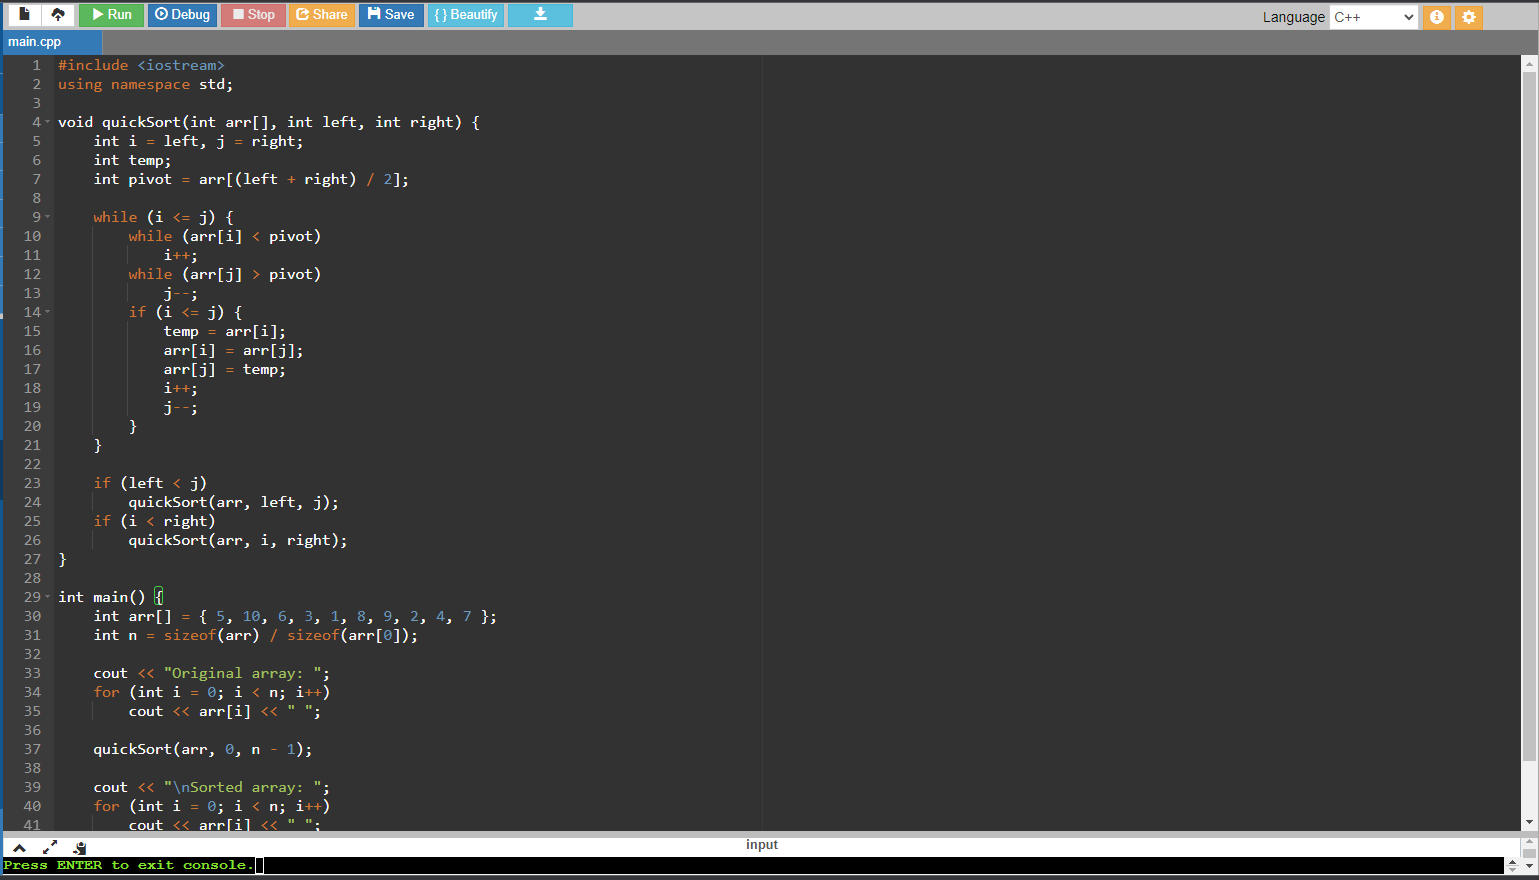
\includegraphics[scale=0.5]{Сортировка.png}
\caption{скриншот программы}\label{fig:par}

\end{figure}
\newpage
\begin{document}
\label{sec:picexample}
\begin{figure}[h]
\centering
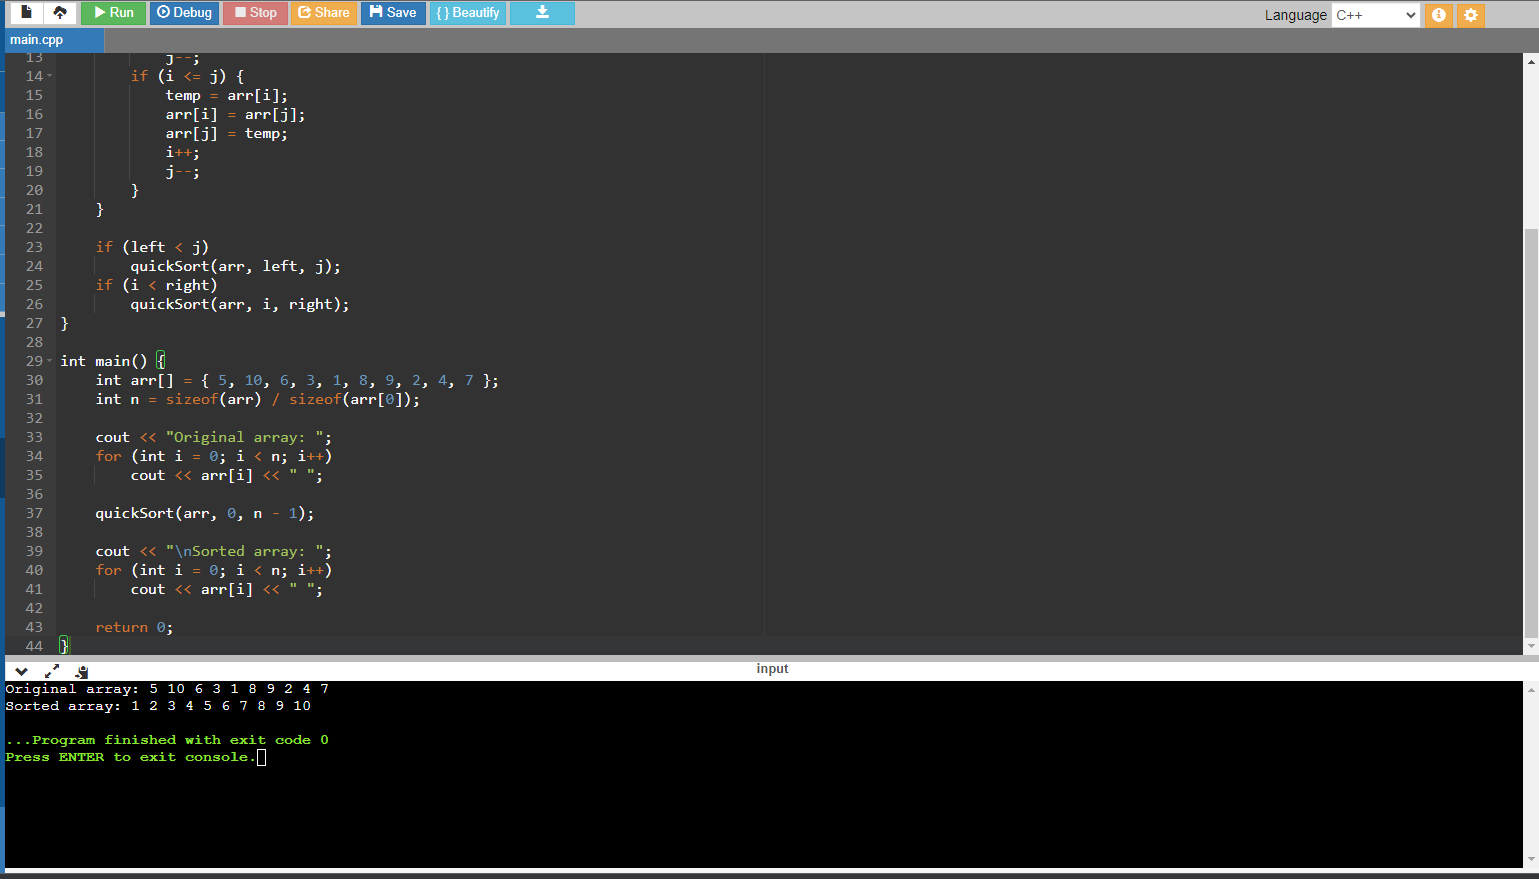
\includegraphics[scale=0.5]{Сортировка2.png}
\caption{скриншот программы}\label{fig:par}

\end{figure}
\newpage
Сортировка слиянием
\begin{document}
\label{sec:picexample}
\begin{figure}[h]
\centering
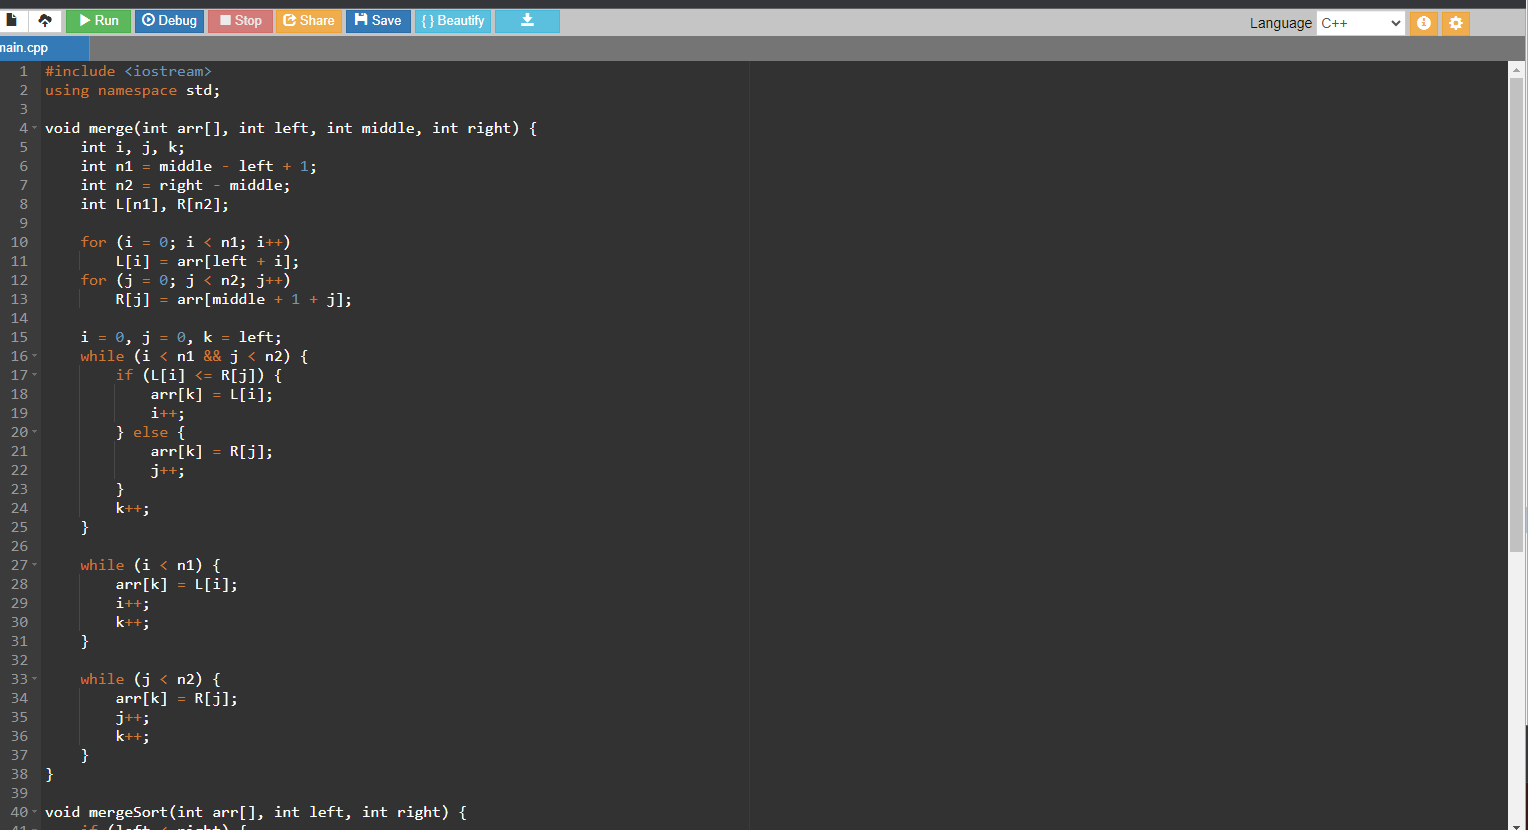
\includegraphics[scale=0.5]{Слияние.png}
\caption{скриншот программы}\label{fig:par}
\end{figure}

\newpage
\begin{document}
\label{sec:picexample}
\begin{figure}[h]
\centering
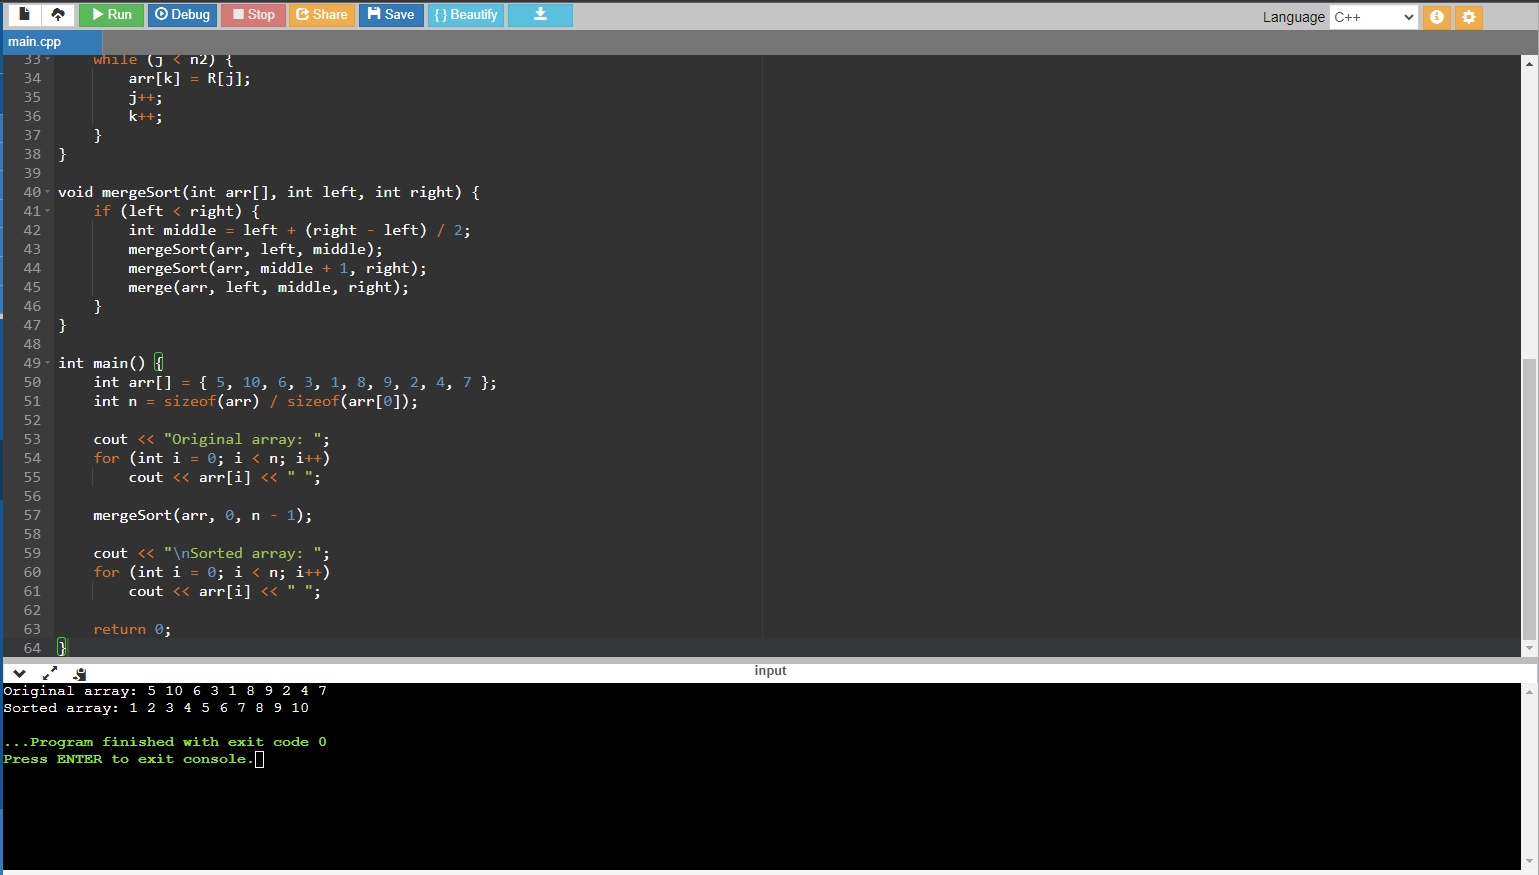
\includegraphics[scale=0.5]{Слияние2.png}
\caption{скриншот программы}\label{fig:par}
\end{figure}

\section{ библиографические ссылки}

Для изучения «внутренностей» \TeX{} необходимо
изучить~\cite{Knuth-2003}, а для использования \LaTeX{} лучше
почитать~\cite{Lvovsky-2003, Voroncov-2005}.

\begin{thebibliography}{9}
\bibitem{Knuth-2003}Кнут Д.Э. Всё про \TeX. \newblock —- Москва: Изд. Вильямс, 2003 г. 550~с.
\bibitem{Lvovsky-2003}Львовский С.М. Набор и верстка в системе \LaTeX{}. \newblock —- 3-е издание, исправленное и дополненное, 2003 г.
\bibitem{Voroncov-2005}Воронцов К.В. \LaTeX{} в примерах. 2005 г.
\end{thebibliography}
\end{document}
\end{document}
\end{document}